\subsection{Etching copper foils}
Growing high quality \textit{h}-BN ad layers on polycrystalline copper foils requires a smooth surface, but as ordered Cu foils exhibit a root-mean-square (RMS) surface roughness $S_q$ of about \SI{218}{\nm}\cite{bin_zhang_low-temperature_2012}. Steep, linear depressions, called striations are fabrication remnants due to the cold rolled foils and observed on the surface\cite{kim_synthesis_2012-1}. Also some manufacturers apply a thin layer of chromium oxide for corrosion protection\cite{bin_zhang_low-temperature_2012}, that has to be removed prior \textit{h}-BN growth. A common procedure to reduce the roughness of a material is to mechanically polish the surface. When a small roughness $S_q$ is needed, electrochemical polishing is an alternative.

A comprehensive overview of \index{electrochemical polishing} electrochemical polishing of Cu surfaces with different etchants  can be found in \cite{jinshan_electrochemical_2004}. The following gives a short introduction in chemical polishing as used for preparation of thin copper foils.\cite{antoine_polishing_1999, lilje_improved_2004, schulz_engeneering_2018}


\label{sec:etching}
\paragraph{Electrochemical cell}
An electrochemical cell used for etching is shown in \autoref{fig:etching-setup}. A beaker is filled with etching solution and two electrodes are immersed. One electrode is the material to be polished (copper foil, working electrode), the other one is the counter electrode (copper in this case, too). Both are placed with \SI{3}{\centi \meter} apart and are oriented parallel. The working electrode has a surface of about \SI{1}{\square \centi \meter}, the counter electrode of about \SI{16}{\square \centi \meter}. 

The beaker is filled with etching solution until both electrodes are covered.

An electric connection is made between working electrode (\SI{0}{\volt} < U < \SI{2}{\volt}) and the power supply. The counter electrode acts as ground. Both electrodes are fixed with alligator clamps to the wires.

\begin{figure}\centering
	\subfigure[Sketch of a typical setup used for electro polishing. A beaker is used to hold the aqueous cell medium. The copper foil and a counter electrode are immersed and connected a the + and - connections of a DC power supply. Image reproduced from \cite{stables_report_2008}]{
		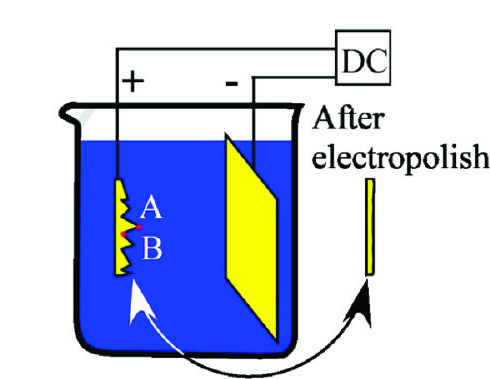
\includegraphics[width=0.4\textwidth]{./images/cm1028854-fig2-d}
		\label{fig:etching-setup}
	} \quad%
	\subfigure[Current-voltage characteristic indicating different phases in the ething and polishing process. While at low voltage etching is the dominant process, a polishing plateau is formed at intermediate voltages. Exceeding a threshold (cusp point) leads to increased formation of excess oxygen in the oxygen pitting regime. \cite{luo_effect_2011}]{
		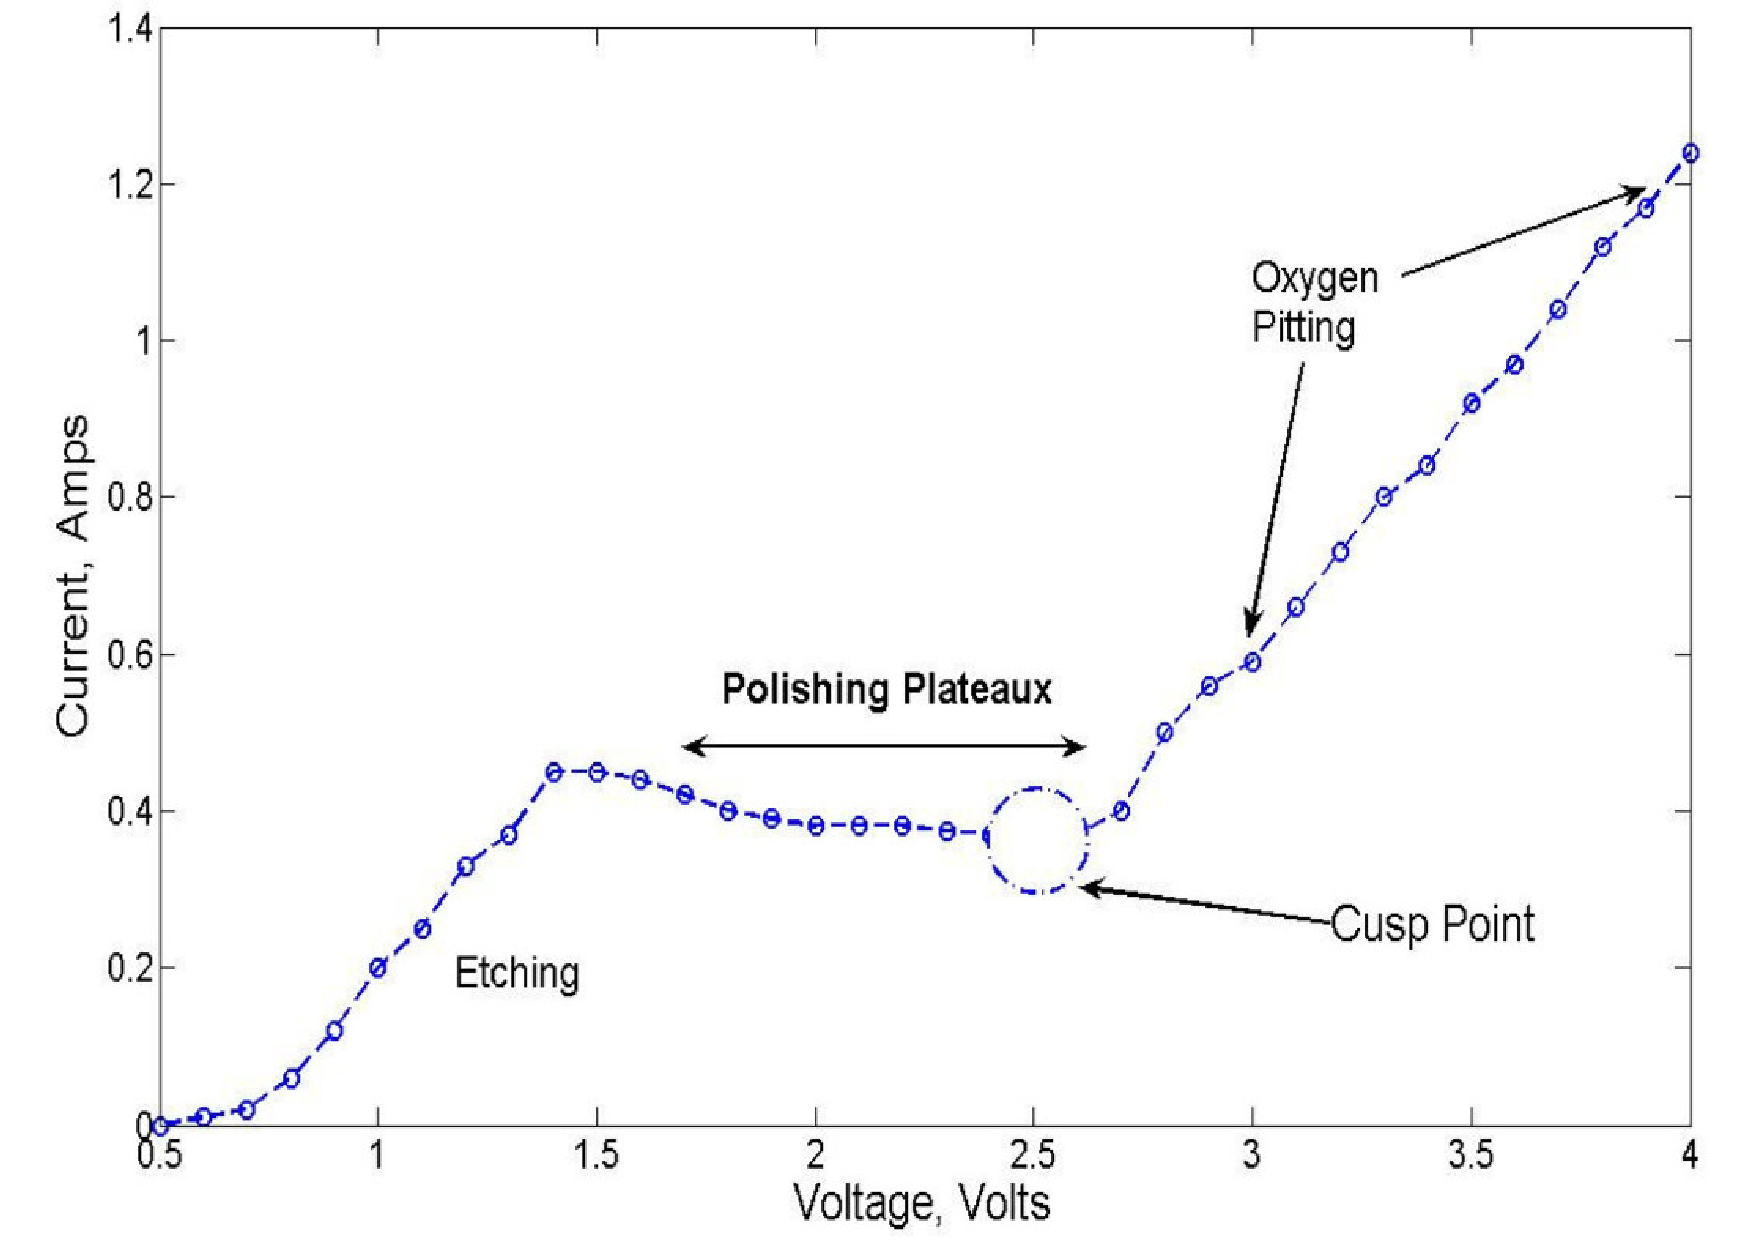
\includegraphics[width=0.4\textwidth]{./images/oxygen-pitting}
		\label{fig:oxygen-pitting}
	}
	\caption{Experimental setup and voltage characteristic used for electrochemical polishing. \subref{fig:etching-setup} In the process the foil is connected as working electrode (+) and opposed by a counter electrode (-). Material is then transported from the working to the counter electrode resulting in a polished foil surface. \subref{fig:oxygen-pitting} Choosing proper voltage and current values in the polishing plateau is important for good results.}
	\label{fig:setup-and-characteristic}
\end{figure}

\paragraph{aqueous etching solution}
Within this work, Cu-foil polishing will be done with the recipe broken down in \autoref{tab:used-etching-solution}. It has several advantages. Since the main goal is the achieve a flat surface, the resulting roughness of the surface is the most important parameter. In contrast to etching recipes without PEG (where oxygen pitting is an issue) and more complex etching recipes (to reduce etching time on exchange of higher surface roughness) a simple etching solution is chosen.

Here we use a simple but efficient etching solution that results in a smooth surface and little etch pits. Pure aqueous ortho-phospheric acid (\SI{85}{\percent}) was investigated \cite{jinshan_electrochemical_2004} and best results are achieved when a voltage of \SI{1.2}{\volt} is applied. The limiting current is \SI{12}{\milli \ampere} and an indication how much material is transported through solution. If now Ethylene-glycol (\SI{5}{\percent} of solutions volume) and deionized water (\SI{25}{\percent}) are added, the potential to etch at remains the same, but the critical current is increased \textcolor{red}{\textbf{due to}}. Not only does the etching rate increase by a factor of 4, the resulting roughness remains the same \SI{5}{\nano \meter}, so both foils are of comparable quality.

Electrons and atoms at the solid surface have higher energy states. Thus some of the atoms on the metal surface may lose electrons to form ions. These ions may also recombine with electrons and become atoms at another moment. Depending on the electronic structures, some metals (such as sodium) are easier than others (such as platinum) to ionize. Copper is relatively stable. Still, some of the surface atoms may be expected to ionize at a moment. The ionization process may be promoted when the metal is in touch with aqueous solution because: 
\begin{itemize}
	\item Metal ions can not move in the metal electrode but can move through the solution, producing electric current in solution with an applied potential
	\item Electrons can move freely in metal solid (electric current in a metal) but can not survive in solution and will quickly recombine with positive ions
	\item Water dipoles and negative ions in solution may drag the surface metal ions into the solution
\end{itemize}

\begin{table}\centering
	\caption{Used etching solutions (compare \cite[130]{jinshan_electrochemical_2004}). Note the change in the removal rate due to higher limiting currents in the solution after adding ethylene-glycol to the solution.}
	\begin{tabular}{lcc}
		& I & II \\ \hline \hline
		$\SI{85}{\percent} H_3PO_4$ & 70 & 100 \\
		Ethylene-gylcol & 5 & 0 \\
		Deionized water & 25 & 0 \\ \hline
		Potential [\SI{}{\V}] & \multicolumn{2}{c}{\SI{1.2}{}} \\
		Current [\SI{}{\mA}] & 46 & 12\\
		Roughness [\SI{}{\nm}] & \multicolumn{2}{c}{\SI{5}{}} \\
		Removal rate [\SI{}{\micro\meter\per\minute}] & \SI{1,0}{} & \SI{0,26}{}\\
	\end{tabular}
	\label{table:used-etching-solutions}
\end{table}

\begin{table}
	\centering
	\caption{Volume and mass fractions for copper foil etching solution.}
	\begin{tabular}{lcccc}
		&unit	&$H_3PO_4$ (85\%)&	EG	&	$H_2O$	\\
		Dichte $\rho$   &[$g/cm^3$]	&	1.87	&	1.11	&	1.00	\\
		$1/rho$		&[$cm^3/g$]	&	0.54	&	0.90	&	1.00	\\
		Anteil 		& \%		&	70	&	5	&	25	\\ \hline
		Menge gesamt    &[$cm^3$]	&		\multicolumn{3}{c}{150} 	\\
		Menge anteilig  &[$cm^3$]	&	105.00	&	7.50	&	37.50	\\
		Gewicht         &[g]		&	196.35	&	8.33	&	37.50	\\
	\end{tabular}
	\label{tab:used-etching-solution}
\end{table}

\paragraph{chemical reaction}\index{electrochemical polishing!chemical reaction}
The electrode connected to the positive pole of the power supply is called anode. And the one connected to the negative pole of the power supply is called cathode. When the applied voltage is high enough, electrons in the anode may be pumped out and the metal atoms on the anode surface will be oxidized (e.g., $Cu - 2e = Cut^{2+}$) and dissolved into the electrolyte solution. Under electrical field, the positive ions (cations) move towards cathode and negative ions (anions) move towards anode. The cations may get electrons and be reduced to neutral atoms (e.g., $Cu^{2-} + 2e = Cu$) again at the cathode surface. Therefore, charge transfer between the two electrodes is carried out via the ion drift in the electrolyte and electron conduction in metal wire. When the working electrode is set to be anode, dissolution is processed at certain potential. Likewise, when the working electrode is set to be cathode, it can result in deposition. For electro polishing of copper, the copper part to be polished is set to be anode while the cathode can be any conductive material (e.g., copper).

The critical potential at which the oxidation / reduction starts to occur is related to the standard redox potential for a specific anode material. The redox potential $E_O$ is a measure (in volts) of the affinity of a substance for electrons - its electro negativity - compared with hydrogen (which is set at \SI{0}{\volt}). Substances more strongly electronegative (i.e., capable of oxidizing or accepting electrons) than hydrogen have positive redox potentials (e.g., $Cu/CU^{2+}$: $E_O = \SI{0.34}{\volt}$). Substances less electronegative (i.e., capable of reducing or giving up electrons) than hydrogen have negative redox potentials (e.g., $Cr^{3+}/Cr^{2+}$: $E_O = \SI{-1.07}{\volt}$)\cite{jinshan_electrochemical_2004}

\paragraph{Voltage-current-characteristic or polarization curve}
\begin{itemize}
	\item[-]On a polycrystalline metal surface there are sites, such as defects and grain boundaries, where atoms are at higher energy states. In addition, due to arbitrary crystal orientation, there are different crystalline planes with different energy states of atoms on the electrode surface. Therefore, atoms at all these different sites and planes have different standard redox potential $E_O$, and as a result, have different dissolution rates.
%	 according to eq. \ref{dissolution-rate}. 
	Such an anodic dissolution will not lead to polishing. Instead, a crystallographic etching is produced (reference [9, 33-35] within \cite{jinshan_electrochemical_2004}). This is true at lower current (or applied potential). This refers to the \textbf{"etching"} regime in \autoref{fig:oxygen-pitting} with $U<\SI{1.5}{\volt}$.
	\item[-]The plateau where the current remains almost constant with increasing voltage is referred to as \textbf{"polishing plateau"}. Overall, the values of iL and EL of the limiting current plateau and the shape of a polarization curve depends on electrolyte solution, anode material, disk rotating speed, solution circulation, temperature, and the distance between anode and cathode.
	Of all the factors, electrolyte is the most important one determining the polarization curve.
	\item[-]With continuing increase of applied potential, other reactions than Cu oxidation and reduction may occur and contribute to the increasing current. These reactions produce $H_2$ and $O_2$ bubbles, which occur at or reach the anode surface. This is known as \textbf{"oxygen pitting"}.
\end{itemize}

\paragraph{oxygen pitting}
Gas (oxygen or hydrogen) bubbles may block $Cu^{2+}$ ion transport and therefore terminate the electrochemical dissolution process on the area inside the bubbles. However, the residual solution on the surface area inside the bubbles may react with Cu atom and result in chemical etching. Depending on the chemical property of the electrolyte solution and the value of current density at which the electrochemical dissolution is occurring, the etching speed can be higher than the rate of electrochemical dissolution. In this case, pits will be produced on the anode and produce a rough surface. If etching does not occur inside the bubbles, or if its speed is slower than that of electrochemical dissolution process, the area inside the bubbles will remain and appears as protruding particles after the electrochemical dissolution process. In either case, a rough surface is produced. Approaches to reduce the effect of oxygen bubbling are done by altering the etching solution with different additives.


\paragraph{Leveling mechanisms}
The etching process relies on the fact that the current density (and thus the etching rate) is higher in protruding regions of the copper foil (Ohmic leveling). As a result the surface of the copper foil will be smoothened \cite{luo_effect_2011}. \textcolor{red}{\textbf{Compare with migration smoothing and diffusion smoothing\cite{jinshan_electrochemical_2004, Huo_Electrochemistry_2007}.}}

It was shown that best results are achieved with following points fulfilled.\cite{Huo_Electrochemical_2003}
\begin{itemize}
	\item The polarization curve shows a wide limiting current plateau (polishing plateau) with low limiting current.
	\item Etching is performed with voltage regulated.
	\item Good circulation of the electrolyte solution to ensure even electro polishing.
	\item Prevent oxygen and hydrogen bubbles created in the etching process to reach the anode surface. Parallel and vertical electrodes are preferred.
	\item Extremely close electrodes increase the effect of ohmic leveling, though gas bubbles reach the anode surface quicker.
\end{itemize}

\paragraph{After etching treatment and storage}
After etching, the samples are rinsed with deionized water to neutralize and remove the remaining etching solution. To seal the samples from ambient moisture and oxygen, they are stored in isopropanol.

%	\paragraph{Removed mass from working electrode}
%	``The current flow of every two electrons results in one copper atom dissolved on the anode and deposited on the cathode. Since $\SI{1}{\ampere}= \SI{1}{\coulomb \second}$, the charge of one electron $e = \SI{1.60218E16}{\coulomb}$, so the number of electrons (per second) in 1 A current is $N_e = \frac{I}{e}$; the number of copper atoms being oxidized or reduced $N_a= \frac{1}{2} N_e= \frac{I}{2e}$, the number of moles $N_m = \frac{N_a}{N_A} = \frac{I}{2eN_A}= \frac{I}{2F}$ where Avogadro's number $N_A = \SI{6.02214E23}{\per \mole}$. The weight of $N_m$ mole copper $W = N_m M = \frac{IM}{2 F}$ where M is the molecular weight of copper. Thats a volume, $V = W / d =\frac{IM}{2 F d}$ where d is the density of copper. Thus a current I produces a dissolution/deposition rate in thickness (\SI{}{\centi\meter \per \second}) \begin{equation} R_d=\frac{M}{2 FdA}I \label{dissolution-rate}\end{equation}
%	where A is the area of the electrode surface.
%	\cite[34]{jinshan_electrochemical_2004}

\subsection{Sample cleaning}
\label{sec:sample-cleaning}
Remaining contaminations 
%in copper (Ag: \SI{0.8}{ppm}, Pb: \SI{0.3}{ppm}, Bi: \SI{0.8}{ppm}) and silver (Cu: \SI{2}{ppm}, Fe: \SI{2}{ppm}, Au: \SI{0.8}{ppm}, Ni: \SI{0.8}{ppm}) 
are removed by repeated sputter\footnote{$U_{accel}=$\SIrange{800}{1000}{\volt}, $T_{sample}\approx \SI{300}{\kelvin}$} and anneal cycles\footnote{Cu: $T_{sample}=\SI{750}{\celsius}$, Ag: $T_{sample}=\SI{450}{\celsius}$, Au\textbackslash Mica: $T_{sample}= \underline{\textbf{get value: 450?}}$} in UHV. Typical cool down temperatures $\leq 5 \frac{K}{s}$ result in a smooth, atomically flat surface with large terrace size. 

While sputter and anneal times are constant ($\approx$ \SIrange{20}{30}{\minute} and $\approx$ \SI{5}{\minute} respectively), the annealing temperature is chosen well below the melting point of the substrate \textcolor{red}{($T_{anneal}=(\textnormal{Cu}: \SI{}{\celsius} \textnormal{Ag}: \textnormal{Au}: )$)}. Before CVD growth of \textit{h}-BN on Cu(111)/Cu-foils the temperature is higher to accommodate for the elevated growth temperatures.

\subsection{\textit{h}-BN growth}
Borazine is used as chemical precursor. It is stored in an evacuated liquid cooler to maintain temperatures below \SI{0}{\celsius} and to ensure no water contaminants are present. Both, elevated temperature and water contaminants, cause the precursor to degenerate quickly in the storage.

\textit{h}-BN is grown by catalytically decomposing the precursor on hot copper substrates in UHV. Typical partial pressures of $\SI{1e-7}{\milli \bar}$ and evaporation times of $\approx \SI{5}{\minute}$ are used while the sample is kept at \SI{750}{\celsius}. After dosage, the temperature is kept constant for another \SI{5}{\minute} to ensure complete decomposition of the precursor and self-healing of defects present during growth. The sample is cooled down with cooling rates $\leq 5 \frac{\SI{}{\kelvin}}{\SI{}{\second}}$ so that no wrinkles are observed at STM temperatures of $\approx \SI{5}{\kelvin}$.

\subsection{Molecule deposition}
%%%%%%%%%%%%%%%%%%%%%%%%%%%%%%%%%%%%%%%%%%%%%%%%%%%%%%%%%%%%%%%%%%%%%%%%%%%%%%%%%%%%%%%%%%%
Molecules are sublimated in UHV by organic molecular beam epitaxy (OMBE). The two/four pocket evaporators resistively heat small quarz crucibles to the chosen temperature while cooling the unused ones with process water (\SI{18}{\celsius}). Prior to deposition molecules undergo a degas precedure to remove unwanted chemicals from the powder. A shutter is used to choose the open pocket and allows for accurate timing of evaporation periods.

\begin{table}\centering
	\caption{Evaporation and degas temperatures used for different molecules.}
	\begin{tabular}{ccrc}
		Name			& Configuration & Degas [\SI{}{\degreeCelsius}]	& Evaporate [\SI{}{\degreeCelsius}]	\\ \hline \hline 
		TPCN			& ---		& ---		& 490		\\ \hline 
		\multirow{3}{*}{TBP}	&single		& \SI{4}{\hour} @ \SI{200}{\degreeCelsius}& 390	\\
		&cis		& ---		& \SI{400}{\degreeCelsius}\\
		&trans		& \SI{4}{\hour} @ \SI{200}{\degreeCelsius} + \SI{1}{\hour} @ \SI{270}{\degreeCelsius}&\SI{370}{\degreeCelsius}\\ \hline 
		\multirow{4}{*}{pyrene} & \multirow{3}{*}{cis}		& \SI{2}{\hour} @ \SI{180}{\degreeCelsius}&	\multirow{3}{*}{250}	\\
		&&+ \SI{1}{\hour} @ \SI{200}{\degreeCelsius} + \SI{10}{\minute} @ \SI{235}{\degreeCelsius} 	&\\
		&&+ \SI{1}{\hour} @ \SI{220}{\degreeCelsius}&\\ 
		&trans		& \SI{1}{\hour} @ \SI{230}{\degreeCelsius}		&\SI{265}{\degreeCelsius}		\\ \hline
		\multirow{3}{*}{DCDB} & \multirow{3}{*}{---} & 1h @ \SIrange{100}{150}{\degreeCelsius}& \multirow{3}{*}{\SIrange{220}{240}{\degreeCelsius}}\\
		&&+\SI{10}{\minute} @ \SI{170}{\degreeCelsius} + \SI{25}{\minute} @ \SI{200}{\degreeCelsius} & \\
		&&+ \SI{40}{\minute} @ \SI{220}{\degreeCelsius}&\\
	\end{tabular}
	\label{tab:molecule-temperatures}
\end{table}